% Source: printed p. 155; PDF p. 164
thì $\operatorname{Path}_G$ không có phần tử nào, nên không phải một monoid (nó thiếu đơn vị). Và nếu $G$ có ít nhất hai đỉnh $a\ne b$, thì các đường đi tầm thường tại $a$ và $b$ đều là phần tử của $\operatorname{Path}_G$, nhưng không thể nối chúng với nhau, nên công thức nhân được đề xuất không được xác định.\hfill$\blacklozenge$

\subsection{Đồng cấu đồ thị}

Một đồ thị $(V,A,\mathrm{src},\mathrm{tgt})$ gồm hai tập hợp và hai hàm. Để có thể so sánh hai đồ thị, hai tập hợp và hai hàm của chúng phải có thể được so sánh theo cách thích hợp.

\noindent\textbf{Định nghĩa 4.3.3.1.} Cho $G=(V,A,\mathrm{src},\mathrm{tgt})$ và $G'=(V',A',\mathrm{src}',\mathrm{tgt}')$ là các đồ thị. Một \emph{đồng cấu đồ thị $f$ từ $G$ đến $G'$}, ký hiệu $f:G\to G'$, gồm hai hàm $f_0:V\to V'$ và $f_1:A\to A'$ sao cho các sơ đồ trong~(4.6) giao hoán:
\stepcounter{equation}
\begin{equation}
\begin{tikzcd}[column sep=large,row sep=large]
A\arrow[r,"f_1"]\arrow[d,"\mathrm{src}"']&A'\arrow[d,"\mathrm{src}'"]\\
V\arrow[r,"f_0"']&V'
\end{tikzcd}
\qquad
\begin{tikzcd}[column sep=large,row sep=large]
A\arrow[r,"f_1"]\arrow[d,"\mathrm{tgt}"']&A'\arrow[d,"\mathrm{tgt}'"]\\
V\arrow[r,"f_0"']&V'
\end{tikzcd}
\tag{4.6}
\end{equation}

\noindent\textit{Nhận xét 4.3.3.2.} Thoạt nhìn các điều kiện~(4.6) có thể có vẻ khó hiểu, nhưng chúng mã hóa một ý tưởng rất quan trọng, nói đại khái là ``mũi tên gắn liền với các đầu mút của chúng''. Trong một ánh xạ đồ thị $G\to G'$, ta không thể tùy tiện đưa một mũi tên của $G$ đến bất kỳ mũi tên nào của $G'$: nó vẫn phải nối những đỉnh mà trước đó nó đã nối. Dưới đây là một ví dụ về ánh xạ không tôn trọng điều kiện này: $a$ nối $1$ với $2$ trước khi ánh xạ, nhưng sau đó thì không:
\begin{center}
\begin{tikzpicture}[>=Stealth,every node/.style={font=\small},vertex/.style={circle,fill,inner sep=1.2pt}]
\draw (-.45,-.4) rectangle (1.65,.65);
\node[vertex,red,label={[red]above:$1$}] (s1) at (0,0) {};
\node[vertex,blue,label={[blue]above:$2$}] (s2) at (1.2,0) {};
\draw[->] (s1)--node[above] {$a$}(s2);
\draw[->] (2,0)--node[above,font=\scriptsize] {$1\mapsto1',\ 2\mapsto2',\ a\mapsto a'$}(5.5,0);
\draw (5.85,-.4) rectangle (9.25,.65);
\node[vertex,red,label={[red]above:$1'$}] (t1) at (6.3,0) {};
\node[vertex,blue,label={[blue]above:$2'$}] (t2) at (7.5,0) {};
\node[vertex,green!55!black,label={[green!55!black]above:$3'$}] (t3) at (8.8,0) {};
\draw[->] (t2)--node[above] {$a'$}(t3);
\end{tikzpicture}
\end{center}
Tính giao hoán của các sơ đồ trong~(4.6) chính là điều cần để bảo đảm rằng một đồng cấu đồ thị được đề xuất xử lý các mũi tên theo cách mong đợi.

\noindent\textit{Ví dụ 4.3.3.3 (Đồng cấu đồ thị).} Cho $G=(V,A,\mathrm{src},\mathrm{tgt})$ và $G'=(V',A',\mathrm{src}',\mathrm{tgt}')$ là các đồ thị được vẽ trong~(4.7):
\stepcounter{equation}
\begin{equation}
\begin{tikzpicture}[>=Stealth,every node/.style={font=\small},vertex/.style={circle,fill,inner sep=1.2pt}]
\draw (-.85,-2.3) rectangle (4.1,.65);\node at (1.8,.95) {$G$};
\node[vertex,red,label={[red]above:$1$}] (a1) at (0,0) {};
\node[vertex,green!55!black,label={[green!55!black]above:$2$}] (a2) at (1.8,0) {};
\node[vertex,red,label={[red]above:$3$}] (a3) at (3.6,0) {};
\node[vertex,label=below:{$4$}] (a4) at (0,-1.8) {};
\node[vertex,blue,label={[blue]above:$5$}] (a5) at (1.8,-1.8) {};
\node[vertex,blue,label={[blue]above:$6$}] (a6) at (3.6,-1.8) {};
\draw[->] (a1)--node[above] {$a$}(a2);\draw[->] (a2)--node[above] {$b$}(a3);
\draw[->] (a1) to[bend right=25] node[left] {$c$}(a4);
\draw[->] (a1) to[bend left=25] node[right] {$d$}(a4);
\draw[->] (a5)--node[above] {$e$}(a6);
\draw[->] (4.4,-.9)--node[above,align=left,font=\scriptsize] {$1\mapsto1',\ 2\mapsto2',$\\$3\mapsto1',\ 4\mapsto4',$\\$5\mapsto5',\ 6\mapsto5'$}(7,-.9);
\draw (7.3,-2.3) rectangle (10.9,.65);\node at (9.1,.95) {$G'$};
\node[vertex,red,label={[red]above:$1'$}] (b1) at (7.8,0) {};
\node[vertex,green!55!black,label={[green!55!black]above:$2'$}] (b2) at (9.6,0) {};
\node[vertex,label=right:{$4'$}] (b4) at (7.8,-1.8) {};
\node[vertex,blue,label={[blue]above:$5'$}] (b5) at (9.6,-1.8) {};
\draw[->] (b1) to[bend left=13] node[above] {$w$}(b2);
\draw[->] (b2) to[bend left=13] node[below] {$x$}(b1);
\draw[->] (b1)--node[left] {$y$}(b4);
\draw[->] (b5) to[out=30,in=-30,looseness=10] node[right] {$z$}(b5);
\end{tikzpicture}
\tag{4.7}
\end{equation}

% Source: printed p. 156; PDF p. 165
Các màu biểu thị lựa chọn hàm $f_0:V\to V'$. Với lựa chọn ấy, điều kiện~(4.6) trong trường hợp này buộc ta chỉ có một lựa chọn duy nhất cho đồng cấu đồ thị $f:G\to G'$. Nói cách khác, trong trường hợp cụ thể này, nơi các mũi tên được đưa đến hoàn toàn được xác định bởi nơi các đỉnh được đưa đến.

\noindent\textit{Bài tập 4.3.3.4.}\keepwithnext
\begin{enumerate}[label=\alph*.]
\item Các mũi tên $a,b,c,d,e$ được đưa đến đâu qua $f_1:A\to A'$ trong sơ đồ~(4.7)?
\item Chọn một phần tử $x\in A$ và kiểm tra rằng nó ứng xử như quy định trong sơ đồ~(4.6).\nobreak\hfill$\diamond$
\end{enumerate}

\noindent\textit{Lời giải 4.3.3.4.}\keepwithnext
\begin{enumerate}[label=\alph*.]
\item Ta có:
\[
f_1(a)=w,\quad f_1(b)=x,\quad f_1(c)=y,\quad f_1(d)=y,\quad f_1(e)=z.
\]
\item Viết dưới dạng phương trình, sơ đồ~(4.6) cho biết với mọi $x\in A=\{a,b,c,d,e\}$, ta cần kiểm tra rằng
\[
\mathrm{src}'\circ f_1(x)=f_0\circ\mathrm{src}(x)
\quad\text{và}\quad
\mathrm{tgt}'\circ f_1(x)=f_0\circ\mathrm{tgt}(x).
\]
Ta kiểm tra hai điều kiện này với $x=a$:
\begin{align*}
\mathrm{src}'(f_1(a))&=\mathrm{src}'(w)=1'=f_0(1)=f_0(\mathrm{src}(a)),\\
\mathrm{tgt}'(f_1(a))&=\mathrm{tgt}'(w)=2'=f_0(2)=f_0(\mathrm{tgt}(a)).
\tag*{$\blacklozenge$}
\end{align*}
\end{enumerate}

\noindent\textit{Bài tập 4.3.3.5.}\keepwithnext

Cho $G$ là một đồ thị, cho $n\in\mathbb{N}$ là một số tự nhiên, và cho $[n]$ là đồ thị chuỗi có độ dài $n$, như trong Ví dụ~4.3.1.8. Một đường đi có độ dài $n$ trong $G$ có phải cùng một thứ với một đồng cấu đồ thị $[n]\to G$ không, hay có những khác biệt tinh tế? Chính xác hơn, có phải luôn có một đẳng cấu giữa tập các đồng cấu đồ thị $[n]\to G$ và tập $\operatorname{Path}_G^{(n)}$ các đường đi có độ dài $n$ trong $G$ không?\hfill$\diamond$

% Source: printed p. 157; PDF p. 166
\noindent\textit{Lời giải 4.3.3.5.}\keepwithnext

Có, một đường đi có độ dài $n$ trong $G$ chính là một đồng cấu đồ thị $[n]\to G$. Phần bàn luận về phạm trù trong Chương~5 làm rõ cách viết sự kiện này một cách hình thức dưới dạng đẳng cấu:
\[
\Hom_{\mathrm{Grph}}([n],G)\cong\operatorname{Path}_G^{(n)}.
\tag*{$\blacklozenge$}
\]

\noindent\textit{Bài tập 4.3.3.6.}\keepwithnext

Cho một đồng cấu đồ thị $f:G\to G'$, có một hàm cảm sinh giữa các tập đường đi của chúng, $\operatorname{Path}(f):\operatorname{Path}(G)\to\operatorname{Path}(G')$.
\begin{enumerate}[label=\alph*.]
\item Giải thích cách hoạt động của nó.
\item Có phải với mọi $n\in\mathbb{N}$, hàm $\operatorname{Path}(f)$ đưa $\operatorname{Path}^{(n)}(G)$ đến $\operatorname{Path}^{(n)}(G')$, hay độ dài đường đi có thể thay đổi trong quá trình này?
\item Giả sử $f_0$ và $f_1$ đơn ánh (nghĩa là qua $f$, không có hai đỉnh khác nhau trong $G$ được đưa đến cùng một đỉnh; tương ứng đối với mũi tên). Điều này có kéo theo $\operatorname{Path}(f)$ cũng đơn ánh không (nghĩa là không có hai đường đi khác nhau được đưa đến cùng một đường đi qua $f$)?
\item Giả sử $f_0$ và $f_1$ toàn ánh (nghĩa là mọi đỉnh trong $G'$ và mọi mũi tên trong $G'$ đều nằm trong ảnh của $f$). Điều này có kéo theo $\operatorname{Path}(f)$ cũng toàn ánh không? Gợi ý: Ít nhất một trong các câu trả lời cho~(b)--(d) là không.\nobreak\hfill$\diamond$
\end{enumerate}

\noindent\textit{Lời giải 4.3.3.6.}\keepwithnext
\begin{enumerate}[label=\alph*.]
\item Cho một đường đi $p$ trong $G$, ta áp dụng $f$ lên nó, từng nút và từng mũi tên, để được một đường đi trong $G'$. Dựa vào Bài tập~4.3.3.5, có một cách nhìn khái quát như sau. Một đường đi trong $G$ là một đồng cấu đồ thị $p:[n]\to G$, với một đồ thị chuỗi $[n]$ có độ dài $n\in\mathbb{N}$. Hợp thành $f\circ p:[n]\to G'$ là một đường đi có độ dài $n$ trong $G'$.
\item Có, $\operatorname{Path}(f)$ đưa $\operatorname{Path}^{(n)}(G)$ đến $\operatorname{Path}^{(n)}(G')$.
\item Có, nó sẽ đơn ánh.
\item Không; có thể $f_0$ và $f_1$ toàn ánh nhưng $\operatorname{Path}(f)$ không toàn ánh. Dưới đây là
% Source: printed p. 158; PDF p. 167
một ví dụ. Xét đồng cấu đồ thị sau $(a\mapsto a'';\ b,b'\mapsto b'';\ c'\mapsto c'')$.\ctfournote{Bản gốc, tr.~158, viết ánh xạ cuối là $c\mapsto c'$, trong khi hình vẽ có đỉnh $c'$ ở đồ thị nguồn và $c''$ ở đồ thị đích. Ký hiệu được sửa thành $c'\mapsto c''$ để khớp với chính các đỉnh của sơ đồ.}
\begin{center}
\begin{tikzpicture}[>=Stealth,every node/.style={font=\small},vertex/.style={circle,fill,inner sep=1.2pt}]
\draw (-.45,-.5) rectangle (2,4.1);\node at (.8,4.4) {$G$};
\node[vertex,label=above:{$a$}] (a) at (0,3.5) {};
\node[vertex,label=right:{$b$}] (b) at (0,1.8) {};
\node[vertex,label=above:{$b'$}] (bp) at (1.5,1.8) {};
\node[vertex,label=right:{$c'$}] (cp) at (1.5,0) {};
\draw[->] (a)--(b);\draw[->] (bp)--(cp);
\draw[->] (2.4,2)--node[above] {$f$}(5,2);
\draw (5.5,-.5) rectangle (6.6,4.1);\node at (6.05,4.4) {$G'$};
\node[vertex,label=above:{$a''$}] (app) at (6,3.5) {};
\node[vertex,label=right:{$b''$}] (bpp) at (6,1.8) {};
\node[vertex,label=right:{$c''$}] (cpp) at (6,0) {};
\draw[->] (app)--(bpp);\draw[->] (bpp)--(cpp);
\end{tikzpicture}
\end{center}
Đồng cấu này toàn ánh trên các đỉnh và mũi tên, nhưng xuất hiện một đường đi mới có độ dài $2$.\nobreak\hfill$\blacklozenge$
\end{enumerate}

\noindent\textit{Bài tập 4.3.3.7.}\keepwithnext

Cho một đồ thị $(V,A,\mathrm{src},\mathrm{tgt})$, cho $\langle\mathrm{src},\mathrm{tgt}\rangle:A\to V\times V$ là hàm được bảo đảm bởi tính chất phổ dụng của tích. Ta có thể hy vọng đúc kết điều kiện~(4.6) cho đồng cấu đồ thị bằng tính giao hoán của một hình vuông duy nhất
\stepcounter{equation}
\begin{equation}
\begin{tikzcd}[column sep=large,row sep=large]
A\arrow[r,"f_1"]\arrow[d,"{\langle\mathrm{src},\mathrm{tgt}\rangle}"']&A'\arrow[d,"{\langle\mathrm{src}',\mathrm{tgt}'\rangle}"]\\
V\times V\arrow[r,"f_0\times f_0"']&V'\times V'
\end{tikzcd}
\tag{4.8}
\end{equation}
Tính giao hoán của sơ đồ~(4.8) có thật sự tương đương với tính giao hoán của các sơ đồ~(4.6) không?\hfill$\diamond$

\noindent\textit{Lời giải 4.3.3.7.}\keepwithnext

Có. Điều này suy ra từ tính chất phổ dụng của tích, Mệnh đề~3.1.1.10.\hfill$\blacklozenge$

\subsubsection*{4.3.3.8\quad Quan hệ hai ngôi và đồ thị}

\noindent\textbf{Định nghĩa 4.3.3.9.} Cho $X$ là một tập hợp. Một \emph{quan hệ hai ngôi trên $X$} là một tập con $R\subseteq X\times X$.

% Source: printed p. 159; PDF p. 168
Nếu $X=\mathbb{N}$ là tập các số tự nhiên,\ctfournote{Bản gốc, tr.~159, gọi $\mathbb{N}$ là ``the set of integers'' (tập các số nguyên). Ký hiệu $\mathbb{N}$ và các bảng minh họa chỉ tập số tự nhiên; thuật ngữ được sửa cho nhất quán với tập hợp được dùng.} thì quan hệ $\le$ thông thường định nghĩa một quan hệ hai ngôi trên $X$: cho $(m,n)\in\mathbb{N}\times\mathbb{N}$, ta đặt $(m,n)\in R$ khi và chỉ khi $m\le n$. Dưới dạng bảng, có thể viết nó như bảng bên trái trong~(4.9):
\stepcounter{equation}
\begin{equation}
\begin{array}{|r|r|}\hline
\multicolumn{2}{|c|}{m\le n}\\\hline m&n\\\hline
0&0\\\hline 0&1\\\hline 1&1\\\hline 0&2\\\hline
1&2\\\hline 2&2\\\hline 0&3\\\hline \vdots&\vdots\\\hline
\end{array}\qquad
\begin{array}{|r|r|}\hline
\multicolumn{2}{|c|}{n=5m}\\\hline m&n\\\hline
0&0\\\hline 1&5\\\hline 2&10\\\hline 3&15\\\hline
4&20\\\hline 5&25\\\hline 6&30\\\hline \vdots&\vdots\\\hline
\end{array}\qquad
\begin{array}{|r|r|}\hline
\multicolumn{2}{|c|}{|n-m|\le1}\\\hline m&n\\\hline
0&0\\\hline 0&1\\\hline 1&0\\\hline 1&1\\\hline
1&2\\\hline 2&1\\\hline 2&2\\\hline \vdots&\vdots\\\hline
\end{array}
\tag{4.9}
\end{equation}
Bảng giữa là quan hệ $\{(m,n)\in\mathbb{N}\times\mathbb{N}\mid n=5m\}\subseteq\mathbb{N}\times\mathbb{N}$, còn bảng bên phải là quan hệ $\{(m,n)\in\mathbb{N}\times\mathbb{N}\mid|n-m|\le1\}\subseteq\mathbb{N}\times\mathbb{N}$.

\noindent\textit{Bài tập 4.3.3.10.}\keepwithnext

Một quan hệ trên $\mathbb{R}$ là một tập con của $\mathbb{R}\times\mathbb{R}$, và ta có thể biểu thị một tập con như vậy của mặt phẳng bằng cách tô vùng. Chọn một chặn sai số $\epsilon>0$ và vẽ quan hệ có thể gọi là \emph{xấp xỉ với sai số $\epsilon$}. Nói cách khác, vẽ quan hệ ``$x$ cách $y$ không quá $\epsilon$''.\hfill$\diamond$

\noindent\textit{Lời giải 4.3.3.10.}\keepwithnext
\begin{center}
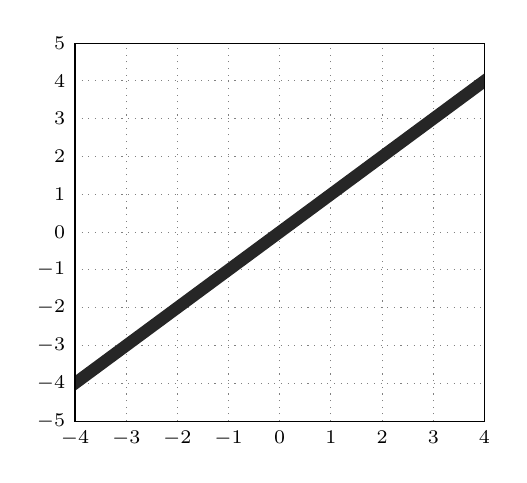
\begin{tikzpicture}[x=.65cm,y=.48cm,every node/.style={font=\scriptsize}]
\draw[step=1,dotted,gray] (-4,-5) grid (4,5);
\begin{scope}\clip (-4,-5) rectangle (4,5);
\fill[black!85] (-4,-4.2)--(4,3.8)--(4,4.2)--(-4,-3.8)--cycle;
\end{scope}
\draw (-4,-5) rectangle (4,5);
\foreach \x in {-4,-3,-2,-1,0,1,2,3,4}{\node[below] at (\x,-5) {$\x$};}
\foreach \y in {-5,-4,-3,-2,-1,0,1,2,3,4,5}{\node[left] at (-4,\y) {$\y$};}
\end{tikzpicture}\quad$\blacklozenge$
\end{center}

% Source: printed p. 160; PDF p. 169
\noindent\textit{Bài tập 4.3.3.11.}\keepwithnext

Nhắc lại rằng~(4.9) dùng các bảng để biểu diễn quan hệ; dùng thuật ngữ về bảng có thể hữu ích khi trả lời một số câu hỏi sau.
\begin{enumerate}[label=\alph*.]
\item Nếu $R\subseteq S\times S$ là một quan hệ hai ngôi, hãy tìm một cách tự nhiên để tạo từ nó một đồ thị $G_R$ có các đỉnh $S$.
\item Tập $A$ các mũi tên trong $G_R$ là gì?
\item Các hàm nguồn và đích $\mathrm{src},\mathrm{tgt}:A\to S$ trong $G_R$ là gì?
\item Xét bảy hàng số trong bảng bên trái của~(4.9), bỏ qua các dấu ba chấm. Vẽ đồ thị tương ứng.
\item Làm tương tự với bảng bên phải của~(4.9).\nobreak\hfill$\diamond$
\end{enumerate}

\noindent\textit{Lời giải 4.3.3.11.}\keepwithnext
\begin{enumerate}[label=\alph*.]
\item Ta có hai phép chiếu $\pi_1,\pi_2:S\times S\to S$ và một ánh xạ bao hàm $i:R\subseteq S\times S$. Do đó ta có một đồ thị
\[
\begin{tikzcd}[column sep=large]
R\arrow[r,shift left=.7ex,"\pi_1\circ i"]\arrow[r,shift right=.7ex,"\pi_2\circ i"']&S
\end{tikzcd}
\]
Ý tưởng là với mỗi hàng trong bảng, ta vẽ một mũi tên từ giá trị ở cột thứ nhất đến giá trị ở cột thứ hai.
\item Đó là $R$, có thể gọi là ``tập các hàng của bảng''.\ctfournote{Bản gốc, tr.~160, viết ``the number of rows in the table'' (số hàng của bảng). Ở đây đang hỏi một tập hợp, và $R$ là tập các cặp được ghi thành hàng; số hàng là lực lượng $|R|$, không phải tập $R$. Vì vậy, lời diễn giải được sửa thành ``tập các hàng''.}
\item Đó là $\pi_1\circ i$ và $\pi_2\circ i$, có thể gọi là ``cột thứ nhất và cột thứ hai của bảng''. Nói cách khác, $G_R:=(S,R,\pi_1\circ i,\pi_2\circ i)$.
\item Bảy mũi tên liền nét trong đồ thị sau tương ứng với bảy hàng được thể hiện trong bảng bên trái; ta thêm ba mũi tên nét đứt để hoàn thiện hình
% Source: printed p. 161; PDF p. 170
(chúng vẫn thỏa mãn quan hệ $\le$).
\begin{center}
\begin{tikzpicture}[>=Stealth,every node/.style={font=\small},vertex/.style={circle,fill,inner sep=1.2pt}]
\node at (1,3) {Một phần của $G_{m\le n}$};
\draw (-.8,-.8) rectangle (2.8,2.7);
\node[vertex,label=above right:{$0$}] (v0) at (0,2) {};
\node[vertex,label=above:{$1$}] (v1) at (2,2) {};
\node[vertex,label=below right:{$2$}] (v2) at (0,0) {};
\node[vertex,label=above right:{$3$}] (v3) at (2,0) {};
\draw[->] (v0)--(v1);\draw[->] (v0)--(v2);\draw[->] (v0)--(v3);\draw[->] (v1)--(v2);
\draw[->,dashed] (v1)--(v3);\draw[->,dashed] (v2)--(v3);
\draw[->] (v0) to[out=140,in=100,looseness=10] (v0);
\draw[->] (v1) to[out=80,in=30,looseness=10] (v1);
\draw[->] (v2) to[out=190,in=260,looseness=10] (v2);
\draw[->,dashed] (v3) to[out=-30,in=-90,looseness=10] (v3);
\end{tikzpicture}
\end{center}
\item Bảy hàng, bảy mũi tên:
\begin{samepage}
\begin{center}
\begin{tikzpicture}[>=Stealth,every node/.style={font=\small},vertex/.style={circle,fill,inner sep=1.2pt}]
\node at (1.6,1.3) {Một phần của $G_{|n-m|\le1}$};
\draw (-.65,-.65) rectangle (3.85,1);
\foreach \i in {0,1,2}{\node[vertex,label=below:{$\i$}] (v\i) at (1.6*\i,0) {};\draw[->] (v\i) to[out=130,in=50,looseness=10] (v\i);}
\draw[->] (v0) to[bend left=8] (v1);\draw[->] (v1) to[bend left=8] (v0);
\draw[->] (v1) to[bend left=8] (v2);\draw[->] (v2) to[bend left=8] (v1);
\end{tikzpicture}
\end{center}
\hfill$\blacklozenge$
\end{samepage}
\end{enumerate}

\noindent\textit{Bài tập 4.3.3.12.}\keepwithnext
\begin{enumerate}[label=\alph*.]
\item Nếu $(V,A,\mathrm{src},\mathrm{tgt})$ là một đồ thị, hãy tìm một cách tự nhiên để tạo từ nó một quan hệ hai ngôi $R\subseteq V\times V$.
\item Với đồ thị $G$ bên trái trong~(4.7), viết quan hệ hai ngôi tương ứng dưới dạng bảng.\nobreak\hfill$\diamond$
\end{enumerate}

\noindent\textit{Lời giải 4.3.3.12.}\keepwithnext
\begin{enumerate}[label=\alph*.]
\item Vì có các hàm $\mathrm{src},\mathrm{tgt}:A\to V$, tính chất phổ dụng của tích cho ta một hàm $\langle\mathrm{src},\mathrm{tgt}\rangle:A\to V\times V$. Đây chưa phải một quan hệ hai ngôi, vì nó có thể không đơn ánh. Vì vậy, cho $R\subseteq V\times V$ là ảnh của $\langle\mathrm{src},\mathrm{tgt}\rangle$; bây giờ ta đã có quan hệ hai ngôi mong muốn.
% Source: printed p. 162; PDF p. 171
\item
\[
\begin{array}{|r|r|}\hline1&2\\\hline1&4\\\hline2&3\\\hline5&6\\\hline\end{array}
\tag*{$\blacklozenge$}
\]
\end{enumerate}

\noindent\textit{Bài tập 4.3.3.13.}\keepwithnext
\begin{enumerate}[label=\alph*.]
\item Cho một quan hệ hai ngôi $R\subseteq S\times S$, bạn biết từ Bài tập~4.3.3.11 cách xây dựng một đồ thị từ nó, và từ Bài tập~4.3.3.12 cách tạo một quan hệ hai ngôi mới từ đồ thị ấy, hoàn thành một vòng đi rồi quay lại. Quan hệ thu được so với quan hệ ban đầu như thế nào?
\item Cho một đồ thị $G=(V,A,\mathrm{src},\mathrm{tgt})$, bạn biết từ Bài tập~4.3.3.12 cách tạo một quan hệ hai ngôi mới từ nó, và từ Bài tập~4.3.3.11 cách xây dựng một đồ thị mới từ quan hệ ấy, hoàn thành vòng đi rồi quay lại theo chiều ngược. Đồ thị thu được so với đồ thị ban đầu như thế nào?\nobreak\hfill$\diamond$
\end{enumerate}

\noindent\textit{Lời giải 4.3.3.13.}\keepwithnext
\begin{enumerate}[label=\alph*.]
\item Nó vẫn như cũ.
\item Nó khác đi. Đồ thị mới $G'$ không bao giờ có hai mũi tên cùng hướng. Nghĩa là trong đồ thị ban đầu $G$, ta có thể có hai mũi tên khác nhau $v_1\to v_2$, nhưng điều này không thể xảy ra trong đồ thị mới. Vì vậy đồ thị cũ và đồ thị mới có cùng số đỉnh, và có một mũi tên $v_1\to v_2$ trong $G$ khi và chỉ khi có một mũi tên $v_1\to v_2$ trong $G'$; nhưng nhiều mũi tên từ một đỉnh đến một đỉnh khác trong $G$ bị gộp thành một mũi tên duy nhất trong $G'$.\nobreak\hfill$\blacklozenge$
\end{enumerate}

\section{Thứ tự}

Người ta thường nghĩ một số tập hợp nhất định vốn có một thứ tự chính tắc. Chẳng hạn, ta có thể nghĩ rằng các số tự nhiên vốn có thứ tự trong đó $3<5$, hoặc các chữ cái trong bảng chữ cái vốn có thứ tự trong đó $b<e$. Nhưng thực ra, chúng ta đặt các thứ tự lên tập hợp, và chỉ là một số thứ tự được dùng phổ biến hơn. Chẳng hạn, ta có thể
% Sentence continues on printed p. 163.
